\chapter{Normal Distribution}
Suppose we are in a probability space well approximated by the multivariate normal (Gaussian) distribution of a random variable $x \in \R^{d_f}$ with mean $\mu$ and non-singular covariance $\Sigma$:
\marginnote{The $d_f=1$ example in the introduction is just where where $\mu$ and $\Sigma$ are scalars.}
\begin{align}
\index{normal ! definition (PDF)}
P_{\text{normal}}(x;\mu,\Sigma) &= \frac{e^{-\frac{1}{2}(x-\mu)^T \Sigma^{-1} (x-\mu)}}{\sqrt{(2\pi)^{d_f} \det{\Sigma}}}  \,,\\
\intertext{where}
\index{normal ! mean $\mu$}
\mu_i &= E(x_i)\,,\\
\intertext{and}
\index{normal ! variance $\Sigma$}
\Sigma_{ij} &= E((x_i-\mu_i)(x_j-\mu_j)) \,.
\end{align}

How lucky is some outcome $x$? From the definition:
\begin{align}
L(x)&=|\Omega(x)|+\frac{1}{2}|\omega(x)| \,,\\
\intertext{where}
\Omega(x) =& \left\{ y \in \R^{d_f} \middle| P_{\text{normal}}(y) > P_{\text{normal}}(x) \right\} \\
          =& \left\{ y \in \R^{d_f} \middle| |\sqrt{\Sigma^{-1}}(y-\mu)| < |\sqrt{\Sigma^{-1}}(x-\mu)| \right\}
\intertext{and}
\omega(x) =& \left\{ y \in \R^{d_f} \middle| |\sqrt{\Sigma^{-1}}(y-\mu)| = |\sqrt{\Sigma^{-1}}(x-\mu)| \right\} \,.
\end{align}
Because $\omega(x)$ has no volume in $\R^{d_f}$,
\begin{equation}
|\omega(x)|=\int_{\omega(x)} P_{\text{normal}}(y;\mu,\Sigma) \, dy = 0 \,.
\end{equation}

 So
\begin{align}
L(x) &=|\Omega(x)|\\
     &=\int_{\Omega(x)} P_{\text{normal}}(y;\mu,\Sigma) \,dy\,.
\end{align}

\marginnote{$\Sigma$ is symmetric and positive definite, and so is its inverse.  The square-root can be computed as a Cholesky decomposition.  In Scilab, \lstinline[language=Scilab]{z=chol(Sigma)'\\(x-mu)}}
By changing variables to $z=\sqrt{\Sigma^{-1}} (x-\mu)$,
\begin{equation}
L(x) = \int_{|z|<R}  P_{\text{normal}}(z;0,I) \, dz \,,
\end{equation}
\marginnote{\lstinline[language=Scilab]{R=norm(z)}}
where $R = |\sqrt{\Sigma^{-1}} (x-\mu)|$.  This can be evaluated in spherical coordinates:
\begin{align}
\label{eq:normal-luck-as-integral}
L(x)    &=\frac{1}{\sqrt{(2\pi)^{d_f}}} \int_{0}^{R} \frac{d_f \pi^{d_f/2}}{\Gamma(\frac{d_f}{2}+1)} r^{d_f-1} e^{-\frac{1}{2} r^2} \, dr \,, \\
\index{luck $L$ ! normal (exact)}
&=\frac{\gamma(n/2,R^2/2)}{\Gamma(n/2)} \,.
\label{eq:luck-normal}
\end{align}
\marginnote{\lstinline[language=Scilab]{L=cdfgam("PQ",R^2/2,df/2,1)}}
The last form uses the lower incomplete gamma function and gamma function, defined to be
\begin{align}
\index{gamma $\gamma$ ! definition}
\gamma(s,x) &= \int_0^{x} t^{s-1} e^{-t} \, dt \\
\index{Gamma $\Gamma$ ! definition}
\Gamma(s) &= \gamma(s,\infty) \,.
\end{align}
For any value of $d_f$, but particularly for large values, we find the following approximation to be very good\marginnote{This comes from a Taylor expansion of the log of the integrand in (\ref{eq:normal-luck-as-integral}), and numerical experimentation on the $1/2$ factor.  The expansion is specifically invalid for $d_f=1$, hence the difference between the general case and the $d_f=1$ case (\ref{eq:normal-1d-luck}).}:
\marginnote{\lstinline[language=Scilab]{Lapprox=0.5*(1+erf(R-sqrt(df-1/2)))}}
\begin{equation}
\label{eq:normal-luck-approx}
\index{luck $L$ ! normal (approximate)}
L(x) \approx \frac{1}{2}\left[1+\erf(|\sqrt{\Sigma^{-1}} (x-\mu)|-\sqrt{d_f-1/2})\right] \,.
\end{equation}
\begin{figure}
  \caption{Exact (blue) vs approximate (red) luck for normal distribution for $d_f=1$, $10$, and $100$.}
  \centering
    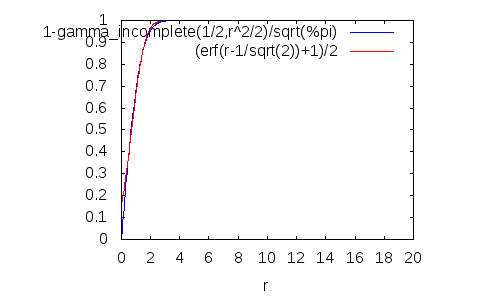
\includegraphics[width=0.75\textwidth]{img/luck1}
    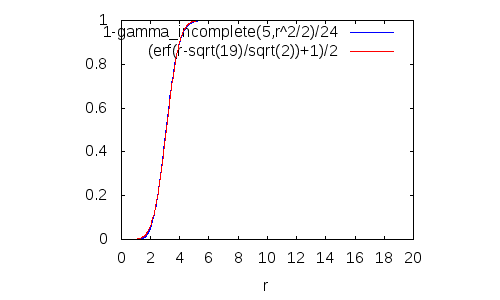
\includegraphics[width=0.75\textwidth]{img/luck10}
    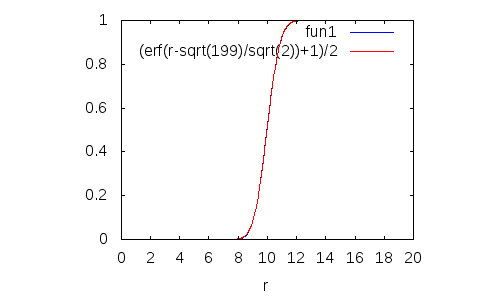
\includegraphics[width=0.75\textwidth]{img/luck100}
\end{figure}

This result has a number of important consequences.  The first is insight into the nature of statistics with many degrees of freedom.  Our expectation before this calculation was that luck would start with $L=0$ at $R=0$ and quickly increase with $R$ before becoming exponentially close to $1$ as $R$ became large.  This is not at all the case:
\begin{quote}
  In large dimensions, normal observations are {\em not} crowded near $x \approx \mu$, but almost certainly ($99.99\%$) within $\pm 3$ of the elliptical shell
  \begin{equation*}
    |\Sigma^{-1/2}(x-\mu)|=\sqrt{d_f-1/2} \,.
  \end{equation*}
\end{quote}
Philosophically, this means nobody should be surprised about not precisely reaching their goals.  If you have enough dimensions to your life to be interesting, you would be very unlucky to be close to the mark on each of them.

\begin{example}{Large $d_f$ normal luck.}
\index{examples ! large $d_f$ normal luck}
We can also use (\ref{eq:normal-luck-approx}) to disprove an observation came from a distribution.  Suppose we have distribution parameters $\mu$ and $\Sigma$, and would like to know if they fit actual observations.  A traditional approach requires a large sample to estimate $\mu$ and $\Sigma$, but we really just need to ask if the observations are surprising (lucky or unlucky).  In large dimensions, numerical experiments suggest one sample is in most cases sufficient to establish practical certainty (probability of error less than $10^{-15}$).
\begin{table}
\caption{\label{tab:normal}Luck from two randomly generated distributions $\mu^{(x)}$ and $\mu^{(y)}$ uniformly chosen in $[0,1]^{100}$, and $\Sigma^{(x)}, \Sigma^{(y)}$ are transposed squares of random $100 \times 100$ matrices.  In each row, $x$ is  a sample from the $\mu^{(x)},\Sigma^{(x)}$, normal distribution, and $y$ is from the $\mu^{(y)},\Sigma^{(y)}$ distribution.  The actual values of $x$ and $y$ are not given, since they are very large (100 numbers each) and uninteresting.}
\begin{tabular}{|S[table-format=2.10]|S[table-format=2.10]|S[table-format=2.10]|S[table-format=2.10]|}
\multicolumn{1}{c}{$L^{(x)}(x)$} &
\multicolumn{1}{c}{$L^{(y)}(x)$} &
\multicolumn{1}{c}{$L^{(x)}(y)$} &
\multicolumn{1}{c}{$L^{(y)}(y)$} \\
\hline
0.5014172020 & 1.0000000000 & 1.0000000000 & 0.8381802641 \\
0.7314212665 & 1.0000000000 & 1.0000000000 & 0.2392581432 \\
0.9825630339 & 1.0000000000 & 1.0000000000 & 0.2716955127 \\
0.0334550807 & 1.0000000000 & 1.0000000000 & 0.4213206259 \\
0.6894299340 & 1.0000000000 & 1.0000000000 & 0.0744616557 \\
0.7363975937 & 1.0000000000 & 1.0000000000 & 0.2940507284 \\
0.3045212967 & 1.0000000000 & 1.0000000000 & 0.7078490147 \\
0.2311115744 & 1.0000000000 & 1.0000000000 & 0.2903130932 \\
0.5852477199 & 1.0000000000 & 1.0000000000 & 0.6369022028 \\
0.2145529261 & 1.0000000000 & 1.0000000000 & 0.2689897874
\end{tabular}
\end{table}

\begin{figure}
  \caption{Histograms of 10,000 luck values in the same distributions as table~\ref{tab:normal}.  Upshot: $y$ values in the $x$ distribution are viewed as extremely lucky and vice-versa, while they are have uniform luck in their own respective distributions.}
  \centering
    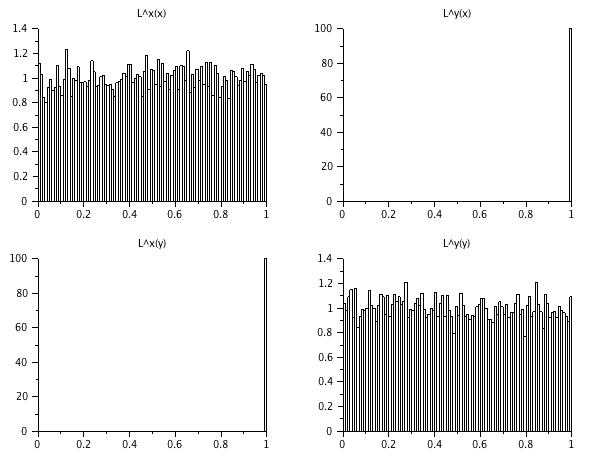
\includegraphics[width=0.75\textwidth]{img/normal}
\end{figure}
\end{example}

\subsection{Combining Normal Luck}
The approximate result (\ref{eq:normal-luck-approx}) leads to a rule for combining (normal) luck:  Suppose there are two independent normal distributions parametrized by $\mu^{(x)}$ , $\Sigma^{(x)}$ of dimension $n_x$, and $\mu^{(y)}$, $\Sigma^{(y)}$ of dimension $n_y$.  What is the luck of a single combined observation $(x,y)$?
\begin{align}
L(x,y) &\approx \frac{1}{2}\left[1+\erf(\sqrt{R_x(x)^2+R_y(y)^2}-\sqrt{d_{fx}+d_{fy}-\frac{1}{2}}) \right] \,,
\intertext{where}
R_x(x) &= \erf^{-1}(2L_x -1)-\sqrt{n_x-\frac{1}{2}} = \sqrt{\left(\Sigma^{(x)}\right)^{-1}} \left(x-\mu^{(x)}\right) \,, \\
R_y(y) &= \erf^{-1}(2L_y -1)-\sqrt{n_y-\frac{1}{2}} = \sqrt{\left(\Sigma^{(y)}\right)^{-1}} \left(y-\mu^{(y)}\right) \,.
\end{align}

The approximations above, which in the limit are exact, lead to the following natural definition:
\begin{definition}{$z$-luck $z_L$.}  For any distribution (not just a normal distribution) with finite mean $\mu=E(x)$ and finite positive definite covariance $\Sigma=E((x-\mu)(x-\mu)^T)$, where $x$ and $\mu$ are $d_f$-dimensional column vectors, it is natural to associate an observation $x$ with the {\em $z$-luck $z_L$}:
\begin{marginlisting}
  df=length(mu);
  z=chol(Sigma)'\(x-mu);
  zl=norm(z)-sqrt(df-1/2);
\end{marginlisting}
\begin{equation}
\index{$z$-luck $z_L$ ! definition}
z_L = \left|\sqrt{\Sigma^{-1}} (x-\mu)\right|-\sqrt{d_f-\frac{1}{2}} \,.
\label{eq:luck-adjusted-z-score}
\end{equation}
\end{definition}

The $z$-luck values from two independent experiments $A$ and $B$ can be combined into one overall score with:
\begin{equation}
\index{$z$-luck $z_L$ ! combine $A \times B$}
\label{eq:zl-combine}
\begin{split}
z_L^{A \times B}=&\sqrt{\left(z_L^A+\sqrt{d_f^A-\frac{1}{2}}\right)^2+\left(z_L^B+\sqrt{d_f^B-\frac{1}{2}}\right)^2}\\
&-\sqrt{d_f^A+d_f^B-\frac{1}{2}} \,,
\end{split}
\end{equation}
and
\begin{equation}
d_f^{A \times B}=d_f^A + d_f^B \,.
\end{equation}

Similarly, $n$ repeated independent experiments $A$ can be combined with
\begin{equation}
\index{$z$-luck $z_L$ ! combine $A^n$}
  \label{eq:zl-combine-n}
\begin{split}
z_L^{A^n}=&\sqrt{\sum_{k=1}^{n}{\left(z_L^{A_k}+\sqrt{d_f^A-\frac{1}{2}}\right)^2}} \\
         &-\sqrt{n\cdot d_f^A - \frac{1}{2}} \,,
\end{split}
\end{equation}
and
\begin{equation}
d_f^{A^n}=n d_f^A \,.
\end{equation}

\begin{definition}{Normal luck $L_N$.}
If the combined dimension $d_f$ is large enough that the overall distribution is well approximated by the normal distribution, then the luck associated with the overall set of observations is well approximated by the {\em normal luck},
\begin{equation}
\index{luck (normal) $L_N$ ! definition}
L_N = \frac{1}{2}\left[1+\erf(z_L)\right] \,.
\end{equation}
\end{definition}

If the distribution is in fact normal, the luck can be computed exactly via,
\begin{equation}
L=\frac{\gamma(\frac{d_f}{2},\frac{1}{2}(z_L+\sqrt{d_f-\frac{1}{2}})^2)}{\Gamma(d_f/2)} \,.
\end{equation}
There is less than a $0.01$ difference between $L_N$ and $L$ for $d_f \geq 22$.

Combining $z$-luck is very useful for understanding the implications of multiple experiments.  If the model is good, the combined $z$-luck value will to stay small (within $\pm 6$) as you combine the outcomes of more experiments.  If it tends to get large or small, there is something wrong in the model.  If $z_L$ tends to negative infinity, this seems to be an indication of a non-stochastic process (it is being gamed), and if $z_L$ tends to positive infinity, the estimates for $\mu$ and/or $\Sigma$ are wrong.  The publication of $z_L$ and $d_f$ for experimental results would be very useful for meta analysis, and $L_N$ or $L$ would be a value much easier to interpret for a lay reader.

\subsection{Scilab Reference Code}

The listings in figures \ref{fig:mnprobln}-\ref{fig:normalluck} give Scilab functions for basic luck calculations for multivariate normal distributions.

\begin{figure}
\caption{\label{fig:mnprobln}Scilab listing to compute the natural log of the probability of multivariate normal outcomes.  $x$ is a $d_f \times n_{\text{samps}}$ matrix of outcomes, $\mu$ is a $d_f \times 1$ column vector of the mean, and $\Sigma$ is a $d_f \times d_f$ covariance matrix.  The result {\tt lnp} is a $1 \times n_{\text{samps}}$ row vector.}
\lstset{language=Scilab}
\begin{lstlisting}
function lnp=mnprobln(x,mu,Sigma)
  [df,nsamps]=size(x);
  sigma=chol(Sigma)';
  one=ones(1,nsamps);  
  z=sigma\(x-mu*one);
  r2=sum(z.^2,'r');
  lnp=-r2/2-(df/2*log(2*%pi)+...
       sum(log(diag(sigma))));
endfunction
\end{lstlisting}
\end{figure}

\begin{figure}
\caption{\label{fig:zluck}Scilab listing to compute the $z$-luck.  $x$ is a $d_f \times n_{\text{samps}}$ matrix of outcomes, $\mu$ is a $d_f \times 1$ column vector of the mean, and $\Sigma$ is a $d_f \times d_f$ covariance matrix.  The result {\tt zl} is a $1 \times n_{\text{samps}}$ row vector.}
\lstset{language=Scilab}
\begin{lstlisting}
function zl=zluck(x,mu,Sigma)
  [df,nsamps]=size(x);
  sigma=chol(Sigma)';
  one=ones(1,nsamps);
  z=sigma\(x-mu*one);
  r=sqrt(sum(z.^2,'r'));
  zl=r-sqrt(df-1/2);
endfunction
\end{lstlisting}
\end{figure}

\begin{figure}
\caption{\label{fig:mnluck}Scilab listing to efficiently compute the luck of multivariate normal outcomes.  $x$ is a $d_f \times n_{\text{samps}}$ of outcomes, $\mu$ is a $d_f \times 1$ column vector of the means, and $\Sigma$ is a $d_f \times d_f$ covariance matrix.  The result $L$ is a $1 \times n_{\text{samps}}$ row vector of the luck associated with each outcome ($U=1-L$).}
\lstset{language=Scilab}
\begin{lstlisting}
function [L,U]=mnluck(x,mu,Sigma)
  [df,nsamps]=size(x);
  one=ones(1,nsamps);
  zl=zluck(x,mu,Sigma);
  r2=(zl+sqrt(df/2)).^2;
  [L,U]=cdfgam("PQ",r2/2,(df/2)*one,one);
endfunction
\end{lstlisting}
\end{figure}

\begin{figure}
\caption{\label{fig:normalluck}Like {\tt mnluck} in figure~\ref{fig:mnluck}, but approximates luck via (\ref{eq:normal-luck-approx}).}
\lstset{language=Scilab}
\begin{lstlisting}
function [L,U]=normalluck(x,mu,Sigma)
  zl=zluck(x,mu,Sigma);
  L=0.5*erfc(-zl);
  U=0.5*erfc(zl);
endfunction
\end{lstlisting}
\end{figure}

\section{Summary}
\begin{itemize}
\item For any distribution with finite mean $\mu$ and co-variance $\Sigma$, a useful parameter is the luck-adjusted $z$-score (\ref{eq:luck-adjusted-z-score}):
  \begin{equation*}
    z_L=\left| \Sigma^{-1/2} (x-\mu) \right| -\sqrt{d_f-\frac{1}{2}} \,.
  \end{equation*}

\item For normal distributions (\ref{eq:luck-normal}),
  \begin{equation*}
  L[{\cal N}(\cdot;\mu,\Sigma)](x)=\frac{\gamma(\frac{d_f}{2},\frac{\left(z_L+\sqrt{d_f-\frac{1}{2}}\right)^2}{2})}{\Gamma\left(\frac{d_f}{2}\right)} \,.
  \end{equation*}

\item For approximately normal distributions (\ref{eq:normal-luck-approx}),
  \begin{equation*}  
    L(x) \approx \frac{1}{2} \left[1+\erf(z_L)\right] \,.
  \end{equation*}

\item Generalizing (\ref{eq:zl-combine}) and (\ref{eq:zl-combine-n}), for $n$ independent experiments $\{A_k\}_{k=1}^{n}$:
  \begin{equation*}
\begin{split}
z_L^{A^n}=&\sqrt{\sum_{k=1}^{n}{\left(z_L^{A_k}+\sqrt{d_f^{A_k}-\frac{1}{2}}\right)^2}} \\
         &-\sqrt{\left(\sum_{k=1}^{n} d_f^{A_k}\right) - \frac{1}{2}} \,,
\end{split}
\end{equation*}
and
\begin{equation*}
d_f^{A^n}=\sum_{k=1}^{n} d_f^{A_k} \,.
\end{equation*}
\item Seeing $|z_L|>Z$ should happen in less than $\frac{2Z}{\sqrt{\pi}} e^{-Z^2}$ fraction of cases.  This can be be a statistical proof (likelihood $O(10^{-45})$) at $Z=10$ with as little as one observation.
\end{itemize}

\section{Exercises}
\begin{enumerate}
\item \label{q:normal-coin} Take the maximum of two fair coin flips (0 or 1), so $\Prob(\max = 0)=1/4$ and $\Prob(\max = 1)=3/4$.  What is the mean $\mu$ and standard deviation $\sigma$ of this distribution?
\item \label{q:normal-coins} Take 10 independent trials like problem \ref{q:normal-coin}.  Compute the value of $z$-luck for each trial.
\item \label{q:normal-luck} Use (\ref{eq:zl-combine-n}) to combine the $z_L$-scores of problem \ref{q:normal-coins}.  What is the overall normalized luck of the trials?
\item \label{q:normal-exp} Now write down what feels like a random sequence of twenty zeros and ones --- don't think too hard about it!  Use these in pairs like problems \ref{q:normal-coin}-\ref{q:normal-coins}.  What was the normal luck of these trials?
\item \label{q:normal-large} Use a stats package to generate 10,000 values $x$ from a 1d normal distribution $A$ with mean of 1 and standard deviation of 1, and 10,000 values $y$ from a distribution $B$ with mean 1.1 and standard deviation 1.1.  Combine the luck to get the overall luck of the 10,000 observations and show $y$ is lucky in $A$ and $x$ is unlucky in $B$.
\end{enumerate}
